Trong đồ án này, em sử dụng kiến trúc lục giác để vận dụng thiết kế hướng miền. Kiến trúc lục giác (Hexagon Architecture) hay còn gọi là kiến trúc cổng và bộ điều hợp (Ports and Adapters Architecture) là một mẫu kiến trúc tạo ra các thành phần ứng dụng được kết nối lỏng lẻo có thể dễ dàng kết nối với môi trường phần mềm của chúng bằng các cổng và bộ điều hợp. Kiến trúc lục giác đặt lớp miền ở trung tâm của phần mềm, cô lập lớp miền và làm cho lớp miền độc lập và ổn định nhất.

\begin{figure}[H]

\centering

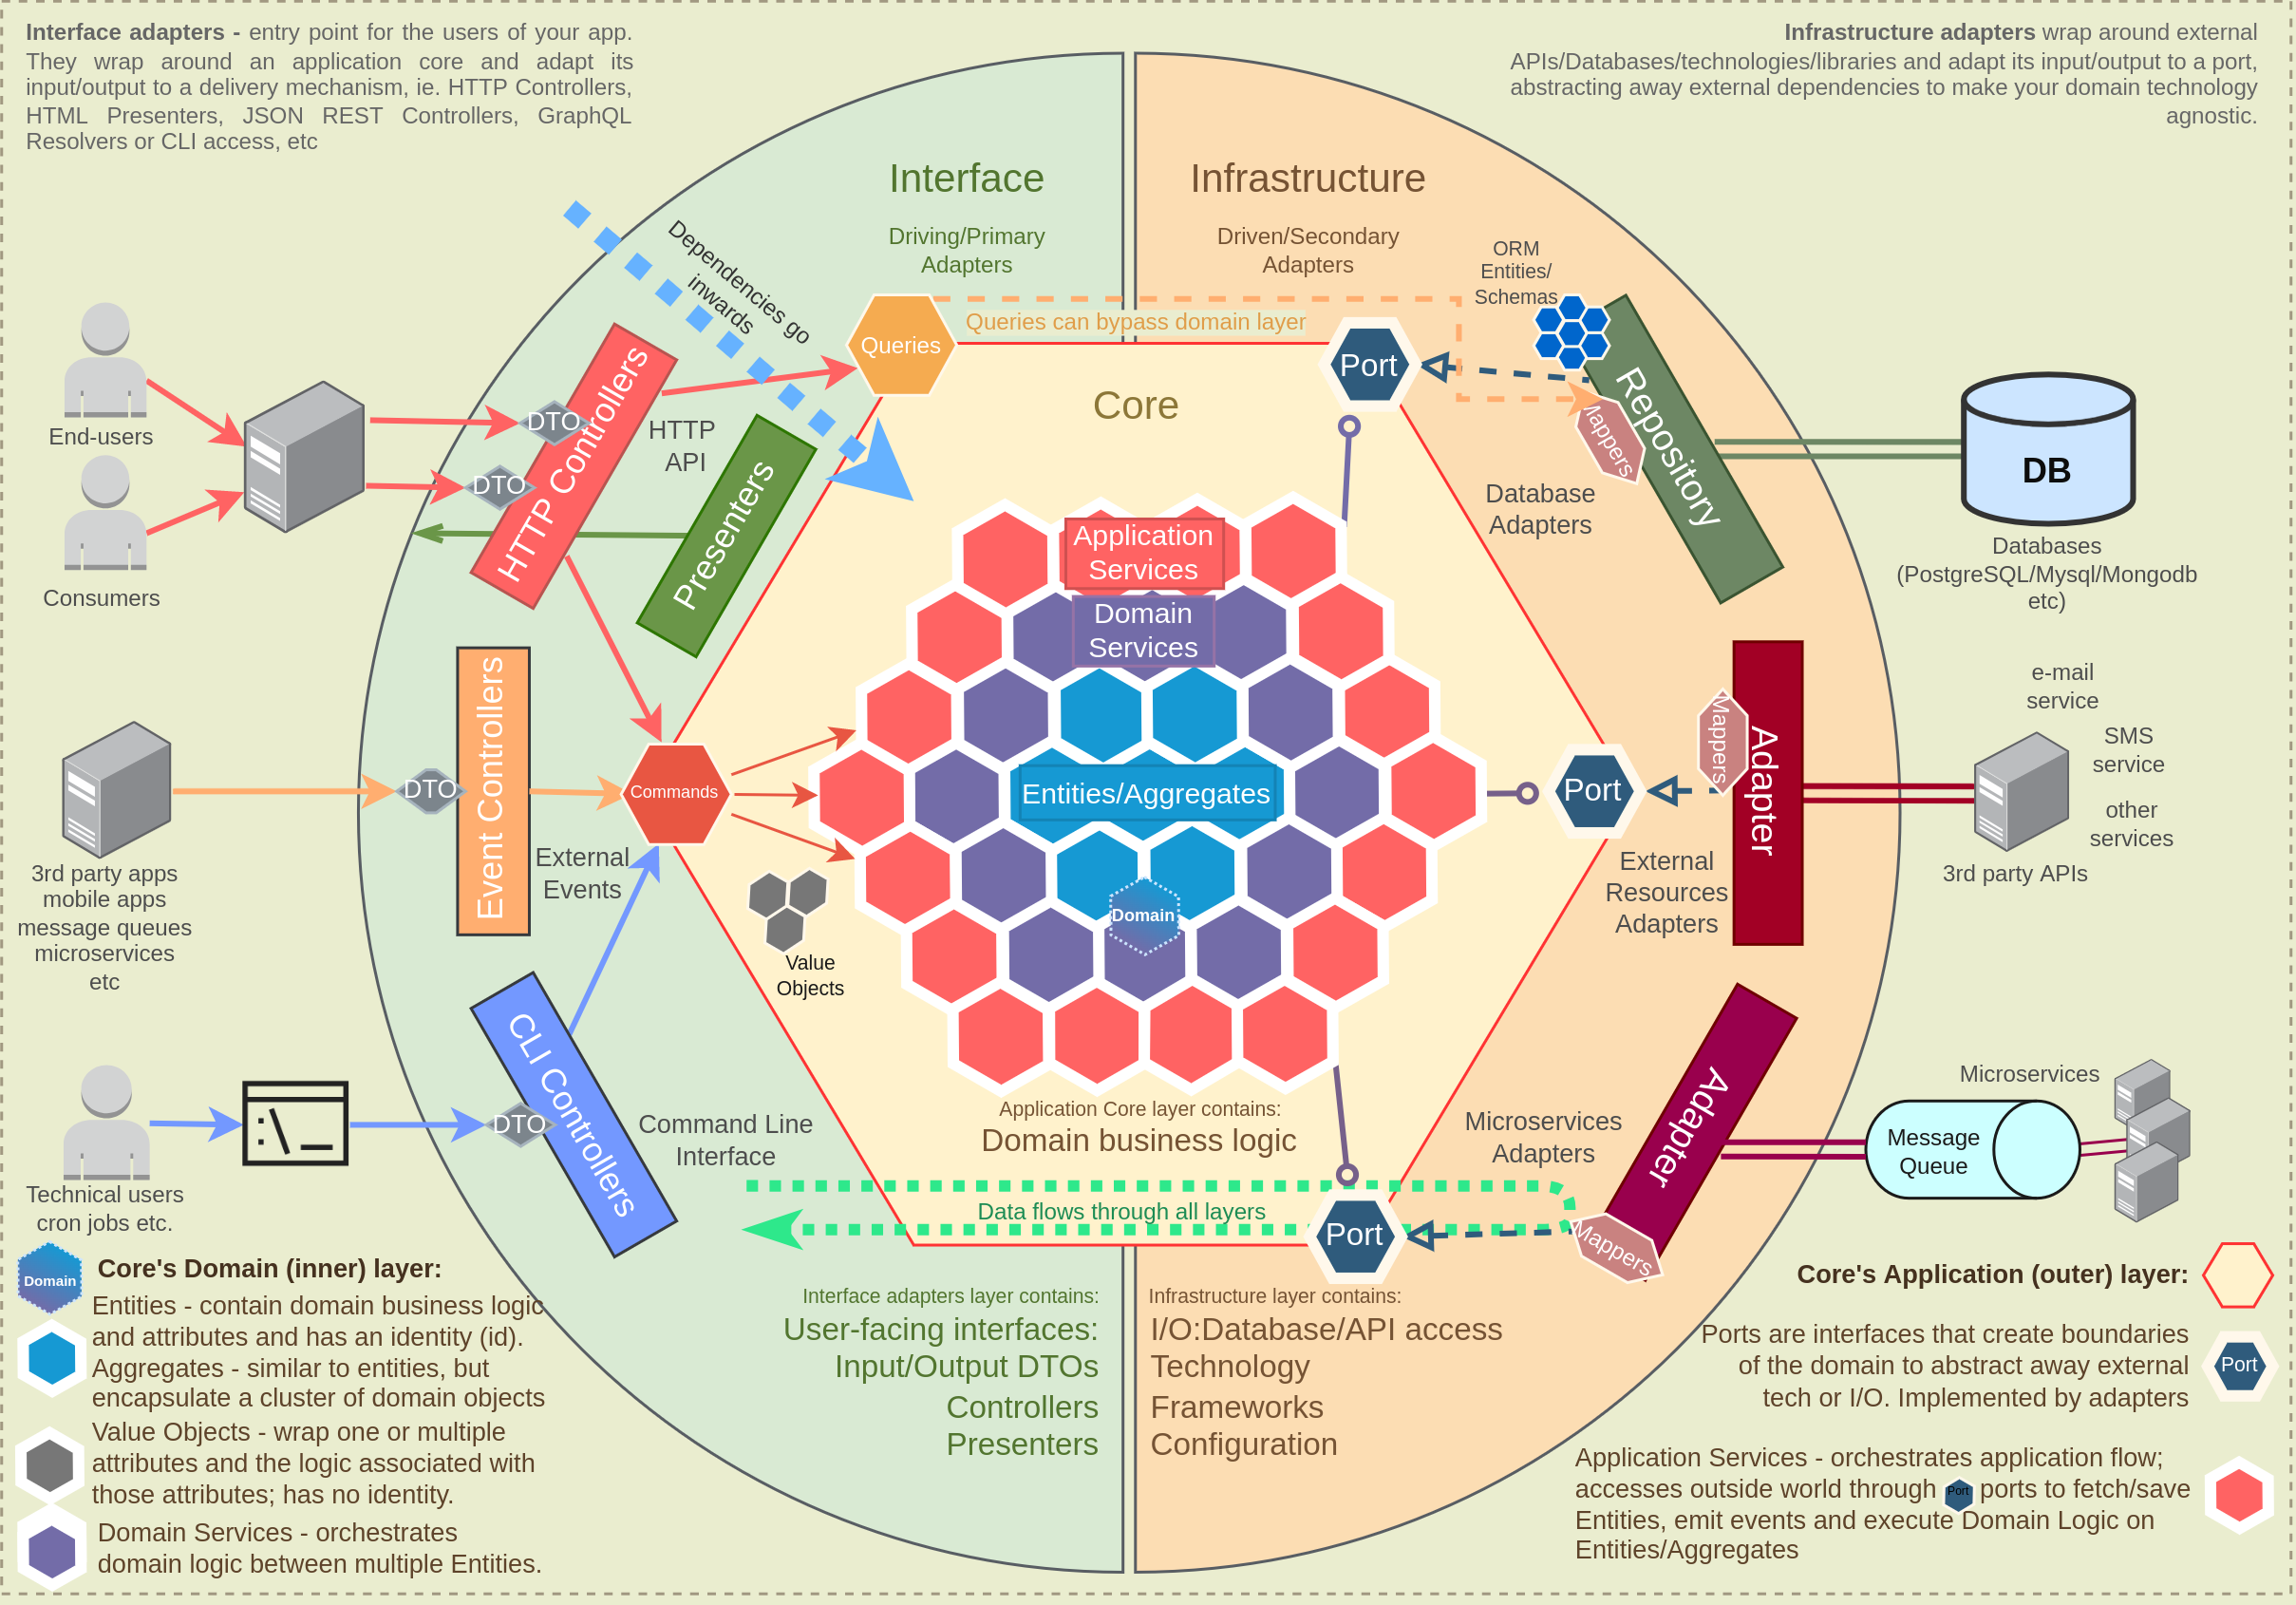
\includegraphics[scale = 0.4]{pictures/_tong_quan_kien_truc_luc_giac/DomainDrivenHexagon.png}

\caption{Tổng quan kiến trúc lục giác}

\end{figure}

Ưu điểm của kiến trúc lục giác là không phụ thuộc vào các khung, công nghệ, cơ sở dữ liệu bên ngoài, \dots Các khung và tài nguyên bên ngoài có thể được cắm/rút mà không tốn nhiều công sức. Từ đó, hệ thống dễ dàng kiểm thử và mở rộng.



\begin{figure}[H]

    \centering
    
    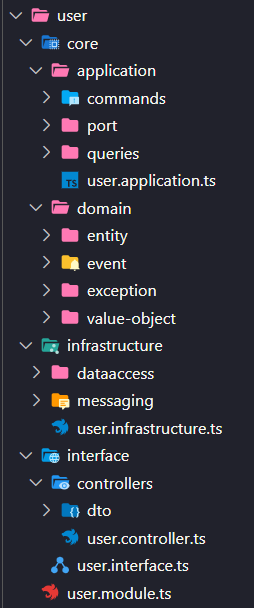
\includegraphics[scale = 0.9]{pictures/_dich_vu_nguoi_dung_nestjs_su_dung_kien_truc_luc_giac/main.png}
    
    \caption{Dịch vụ người dùng NestJS sử dụng kiến trúc lục giác}
    
    \end{figure}
% 35

% 00:02:04, 410 --> 00:02:08, 763

% Kiến trúc lục giác còn được gọi là Cổng và Bộ điều hợp.

% 36

% 00:02:09, 750 --> 00:02:12, 660

% Ý tưởng chính là chia

% phần mềm thành hai

% 37

% 00:02:12, 660 --> 00:02:17, 660

% phần chính, thông tin

% chi tiết và bên ngoài.

% 38

% 00:02:18, 900 --> 00:02:21, 840

% Thông tin chi tiết sẽ là lớp

% 39

% 00:02:21, 840 --> 00:02:23, 943

% miền chứa logic nghiệp vụ.

% 40

% 00:02:25, 200 --> 00:02:27, 660

% Những phần này sẽ

% được phát triển trước tiên

% 41

% 00:02:27, 660 --> 00:02:30, 453

% và không phụ thuộc

% vào bất kỳ lớp nào khác.

% 42

% 00:02:31, 890 --> 00:02:34, 170

% Vì vậy, nó phải là

% lớp độc lập và ổn định

% 43

% 00:02:34, 170 --> 00:02:38, 373

% nhất vì nó là trái tim

% của phần mềm của bạn.

% 44

% 00:02:40, 200 --> 00:02:44, 040

% Bên ngoài sẽ bao

% gồm tất cả các lớp phụ

% 45

% 00:02:44, 040 --> 00:02:47, 970

% thuộc như API được

% người dùng cuối gọi,

% 46

% 00:02:47, 970 --> 00:02:50, 430

% cơ sở dữ liệu được sử dụng để

% 47

% 00:02:50, 430 --> 00:02:52, 233

% duy trì kết quả

% của logic nghiệp vụ,

% 48

% 00:02:53, 250 --> 00:02:55, 110

% hàng đợi tin nhắn

% hoặc kho sự kiện để

% 49

% 00:02:55, 110 --> 00:02:58, 203

% gửi thông báo đến

% các hệ thống khác,

% 50

% 00:02:59, 070 --> 00:03:01, 560

% một dịch vụ bên ngoài cần

% 51

% 00:03:01, 560 --> 00:03:03, 390

% được gọi từ lớp nghiệp vụ,

% 52

% 00:03:03, 390 --> 00:03:05, 580

% hoặc thậm chí bất kỳ

% framework nào được sử

% 53

% 00:03:05, 580 --> 00:03:08, 223

% dụng trong phần mềm

% như Spring Framework.

% 54

% 00:03:09, 240 --> 00:03:13, 593

% Tất cả những phần bên ngoài này thực ra không phải là phần mềm của bạn.

% 55

% 00:03:14, 550 --> 00:03:18, 483

% Chúng nên được coi như phần bổ trợ cho phần mềm của bạn.

% 56

% 00:03:20, 070 --> 00:03:23, 070

% Vì vậy nguyên tắc chính của

% 57

% 00:03:23, 070 --> 00:03:25, 020

% Kiến trúc lục

% giác là cô lập miền

% 58

% 00:03:25, 020 --> 00:03:27, 483

% khỏi bất kỳ sự phụ thuộc nào trong số này.

% 59

% 00:03:28, 830 --> 00:03:32, 100

% Nó sẽ tạo ra các

% ứng dụng có thể kiểm

% 60

% 00:03:32, 100 --> 00:03:34, 620

% tra dễ dàng với logic

% nghiệp vụ riêng biệt,

% 61

% 00:03:34, 620 --> 00:03:37, 653

% từ cơ sở hạ tầng và nguồn dữ liệu.

% 62

% 00:03:39, 390 --> 00:03:43, 080

% Kiến trúc lục giác

% được phát minh

% 63

% 00:03:43, 080 --> 00:03:44, 763

% vào năm 2005 bởi

% Alistair Cockburn.

% 64

% 00:03:45, 630 --> 00:03:48, 660

% Ông mô tả nó là cho phép

% ứng dụng được điều khiển

% 65

% 00:03:48, 660 --> 00:03:52, 470

% một cách bình đẳng bởi

% người dùng, chương trình,

% 66

% 00:03:52, 470 --> 00:03:55, 560

% kiểm tra tự động hoặc tập lệnh hàng loạt.

% 67

% 00:03:55, 560 --> 00:03:58, 860

% Và được phát triển và thử nghiệm riêng biệt

% 68

% 00:03:58, 860 --> 00:04:02, 823

% từ các thiết bị và cơ sở dữ liệu thời gian chạy cuối cùng của nó.

% 69

% 00:04:05, 310 --> 00:04:07, 743

% Ở đây bạn thấy hai loại bộ điều hợp.

% 70

% 00:04:09, 720 --> 00:04:13, 830

% Bộ điều hợp là các thành phần có thể hoán đổi cho nhau.

% 71

% 00:04:13, 830 --> 00:04:16, 019

% Bộ điều hợp chính là bộ điều hợp

% 72

% 00:04:16, 019 --> 00:04:19, 709

% sử dụng logic cốt

% lõi trong lớp miền.

% 73

% 00:04:19, 709 --> 00:04:23, 880

% Chúng sử dụng các

% cổng đầu vào để gọi các

% 74

% 00:04:23, 880 --> 00:04:26, 193

% triển khai được xác

% định trong lớp miền.

% 75

% 00:04:28, 320 --> 00:04:31, 500

% Trong khi Bộ điều hợp phụ được

% 76

% 00:04:31, 500 --> 00:04:33, 540

% triển khai trong các

% mô-đun bên ngoài

% 77

% 00:04:33, 540 --> 00:04:35, 643

% như cơ sở dữ liệu hoặc hàng đợi tin nhắn.

% 78

% 00:04:36, 900 --> 00:04:38, 430

% Trong kiến ​​trúc này, đầu vào

% 79

% 00:04:38, 430 --> 00:04:41, 190

% của người dùng

% được xử lý bởi một

% 80

% 00:04:41, 190 --> 00:04:46, 090

% hoặc nhiều Bộ điều hợp chính và được chuyển đến logic lõi

% 81

% 00:04:47, 220 --> 00:04:49, 560

% và logic cốt lõi chỉ tương

% 82

% 00:04:49, 560 --> 00:04:51, 843

% tác với bộ điều hợp phụ này.

% 83

% 00:04:52, 830 --> 00:04:55, 410

% Sau đó đầu ra của logic cốt lõi.

% 84

% 00:04:55, 410 --> 00:04:57, 540

% Chúng tôi quay

% lại với người dùng

% 85

% 00:04:57, 540 --> 00:04:59, 673

% cuối, sử dụng lại

% Bộ điều hợp chính.

% 86

% 00:05:00, 780 --> 00:05:04, 200

% Nhận ra rằng chúng

% tôi sử dụng các

% 87

% 00:05:04, 200 --> 00:05:06, 240

% giao diện để tích hợp

% đầu vào và đầu ra,

% 88

% 00:05:06, 240 --> 00:05:08, 940

% và Dependency Insert

% được sử dụng để vượt qua

% 89

% 00:05:08, 940 --> 00:05:12, 480

% quá trình triển khai

% các bộ điều hợp thứ cấp

% 90

% 00:05:12, 480 --> 00:05:14, 550

% đến logic cốt lõi và Bộ điều

% 91

% 00:05:14, 550 --> 00:05:18, 933

% hợp chính ra bên ngoài như API.

% 92

% 00:05:20, 168 --> 00:05:21, 990

% Có rất nhiều lợi ích khi sử dụng

% 93

% 00:05:21, 990 --> 00:05:25, 500

% Kiến trúc sạch và hình lục giác.

% 94

% 00:05:25, 500 --> 00:05:28, 410

% Trước hết, bạn nên hiểu rằng nó

% 95

% 00:05:28, 410 --> 00:05:31, 863

% chủ yếu tốt cho các

% ứng dụng lâu dài.

% 96

% 00:05:32, 790 --> 00:05:35, 880

% Nó sẽ cho phép để lại càng nhiều

% 97

% 00:05:35, 880 --> 00:05:39, 573

% tùy chọn mở càng lâu càng tốt.

% 98

% 00:05:40, 590 --> 00:05:43, 890

% Với những ứng dụng như vậy,

% bạn sẽ nhận ra rằng mình luôn

% 99

% 00:05:43, 890 --> 00:05:47, 640

% cần phải thích ứng với những

% thay đổi của công nghệ mới

% 100

% 00:05:47, 640 --> 00:05:50, 970

% để giữ cho phần mềm của bạn ở trạng thái tốt.

% 101

% 00:05:50, 970 --> 00:05:53, 100

% Như đã đề cập, những

% thay đổi này không

% 102

% 00:05:53, 100 --> 00:05:55, 710

% liên quan gì đến logic

% kinh doanh của bạn.

% 103

% 00:05:55, 710 --> 00:05:59, 700

% Ví dụ: ngày nay bạn có thể sử dụng cơ sở dữ liệu quan hệ.

% 104

% 00:05:59, 700 --> 00:06:01, 410

% Ngày mai bạn có thể muốn áp dụng

% 105

% 00:06:01, 410 --> 00:06:03, 930

% cho một cơ sở dữ

% liệu quan hệ khác

% 106

% 00:06:03, 930 --> 00:06:07, 110

% hoặc thậm chí đến cơ sở dữ liệu không có SQL.

% 107

% 00:06:07, 110 --> 00:06:07, 980

% Trong trường hợp này, bằng cách

% 108

% 00:06:07, 980 --> 00:06:11, 190

% tách biệt logic

% kinh doanh của bạn

% 109

% 00:06:11, 190 --> 00:06:14, 523

% bạn sẽ có thể dễ dàng thay đổi nguồn dữ liệu của mình.

% 110

% 00:06:16, 290 --> 00:06:19, 230

% Trong một kiến ​​trúc lớp truyền thống.

% 111

% 00:06:19, 230 --> 00:06:21, 570

% Nói với ba lớp, giao diện người

% 112

% 00:06:21, 570 --> 00:06:25, 350

% dùng, lớp kinh doanh và dữ liệu.

% 113

% 00:06:25, 350 --> 00:06:28, 560

% Nó sẽ có tất cả các điểm phụ

% 114

% 00:06:28, 560 --> 00:06:30, 450

% thuộc của chúng

% tôi theo một hướng.

% 115

% 00:06:30, 450 --> 00:06:34, 530

% Mỗi lớp trên tùy thuộc vào lớp dưới.

% 116

% 00:06:34, 530 --> 00:06:36, 300

% Vì vậy, trong trường

% hợp đó, lớp nghiệp

% 117

% 00:06:36, 300 --> 00:06:38, 223

% vụ của bạn sẽ phụ

% thuộc vào lớp dữ liệu.

% 118

% 00:06:39, 540 --> 00:06:42, 300

% Điều này sẽ ngăn

% việc thay đổi lớp dữ

% 119

% 00:06:42, 300 --> 00:06:44, 493

% liệu mà không chạm

% vào lớp nghiệp vụ.

% 120

% 00:06:46, 440 --> 00:06:49, 200

% Với Kiến trúc sạch

% và lục giác, tất cả các

% 121

% 00:06:49, 200 --> 00:06:53, 310

% phần phụ thuộc sẽ

% trỏ đến lớp nghiệp vụ

% 122

% 00:06:53, 310 --> 00:06:55, 530

% làm cho lớp nghiệp

% vụ trở nên độc

% 123

% 00:06:55, 530 --> 00:06:58, 110

% lập với bất kỳ sự

% phụ thuộc nào khác.

% 124

% 00:06:58, 110 --> 00:06:59, 400

% Trong các bài giảng sắp tới,

% 125

% 00:06:59, 400 --> 00:07:02, 460

% Tôi sẽ bắt đầu viết microservice

% 126

% 00:07:02, 460 --> 00:07:04, 920

% đầu tiên bằng

% Kiến trúc sạch này.

% 127

% 00:07:04, 920 --> 00:07:06, 510

% Sau đó, bạn sẽ thấy

% các cổng và bộ điều hợp

% 128

% 00:07:06, 510 --> 00:07:10, 110

% sẽ giúp đảo ngược sự

% phụ thuộc như thế nào

% 129

% 00:07:10, 110 --> 00:07:12, 813

% và làm cho logic nghiệp vụ trở nên độc lập.

% 130

% 00:07:13, 680 --> 00:07:16, 920

% Tôi sẽ sử dụng Nguyên tắc đảo

% 131

% 00:07:16, 920 --> 00:07:18, 810

% ngược phụ thuộc để

% thực hiện điều này.

% 132

% 00:07:18, 810 --> 00:07:22, 920

% Với Nguyên tắc đảo ngược

% phụ thuộc và Đa hình, mọi

% 133

% 00:07:22, 920 --> 00:07:27, 210

% phụ thuộc mã nguồn đều có

% thể dễ dàng được đảo ngược

% 134

% 00:07:27, 210 --> 00:07:29, 070

% và các module cấp thấp như

% 135

% 00:07:29, 070 --> 00:07:32, 190

% lớp nguồn dữ liệu

% sẽ là các plugin

% 136

% 00:07:32, 190 --> 00:07:35, 313

% đến các mô-đun cấp cao như logic nghiệp vụ.

% 137

% 00:07:37, 050 --> 00:07:38, 250

% Trong bài giảng tiếp theo,

% 138

% 00:07:38, 250 --> 00:07:40, 410

% Tôi sẽ sử dụng sơ

% đồ để giải thích sự đảo

% 139

% 00:07:40, 410 --> 00:07:43, 680

% ngược phụ thuộc này

% trên microservice đầu tiên,

% 140

% 00:07:43, 680 --> 00:07:45, 363

% đó là dịch vụ đặt hàng.

% 141

% 00:07:48, 510 --> 00:07:50, 880

% Với Clean Architecture,

% bạn sẽ có thể trì hoãn các

% 142

% 00:07:50, 880 --> 00:07:55, 113

% quyết định triển khai của

% tất cả các phần phụ thuộc.

% 143

% 00:07:56, 220 --> 00:07:59, 040

% Và chỉ có thể triển khai

% logic kinh doanh của

% 144

% 00:07:59, 040 --> 00:08:01, 230

% bạn mà không cần suy

% nghĩ bất kỳ hạn chế nào

% 145

% 00:08:01, 230 --> 00:08:03, 693

% của bất kỳ nguồn dữ liệu hoặc khung công tác nào.

% 146

% 00:08:05, 280 --> 00:08:08, 610

% Bạn thậm chí có thể kiểm

% tra hoàn toàn logic kinh

% 147

% 00:08:08, 610 --> 00:08:11, 043

% doanh của mình bằng cách

% đánh dấu các phần phụ thuộc.

% 148

% 00:08:12, 630 --> 00:08:14, 843

% Ngoài ra, như đã

% đề cập, bạn có thể

% 149

% 00:08:14, 843 --> 00:08:18, 750

% thay thế bất kỳ triển

% khai bộ điều hợp nào

% 150

% 00:08:18, 750 --> 00:08:21, 063

% mà không cần chạm vào lớp nghiệp vụ.

% 151

% 00:08:22, 560 --> 00:08:25, 830

% Và bạn có thể duy

% trì từng lớp riêng biệt

% 152

% 00:08:25, 830 --> 00:08:27, 663

% mà không ảnh hưởng

% đến các lớp khác.

% 153

% 00:08:28, 740 --> 00:08:31, 380

% Nó cũng sẽ cho phép

% tách biệt việc phát triển

% 154

% 00:08:31, 380 --> 00:08:34, 472

% và triển khai các lớp

% và mô-đun khác nhau.

% 155

% 00:08:35, 970 --> 00:08:38, 850

% Hơn nữa, các lớp tách biệt

% 156

% 00:08:38, 850 --> 00:08:41, 580

% đương nhiên dễ hiểu hơn

% 157

% 00:08:41, 580 --> 00:08:45, 063

% bởi vì mỗi người trong số họ tập trung vào logic riêng của mình.

% 158

% 00:08:46, 890 --> 00:08:49, 350

% Khi tôi đếm tất cả những

% 159

% 00:08:49, 350 --> 00:08:50, 183

% lợi ích này, bạn có thể nghĩ,

% 160

% 00:08:50, 183 --> 00:08:52, 020

% có bất lợi nào khi sử dụng

% 161

% 00:08:52, 020 --> 00:08:52, 970

% những kiến ​​trúc này không?

% 162

% 00:08:54, 090 --> 00:08:55, 920

% Trong phát triển phần mềm, mọi

% 163

% 00:08:55, 920 --> 00:08:58, 623

% giải pháp đều có

% ưu và nhược điểm.

% 164

% 00:08:59, 760 --> 00:09:02, 400

% Với Kiến trúc sạch

% hoặc lục giác, cái

% 165

% 00:09:02, 400 --> 00:09:06, 300

% giá bạn phải trả là

% viết nhiều mã hơn.

% 166

% 00:09:06, 300 --> 00:09:09, 600

% Đôi khi bạn thậm chí

% cần sao chép một số mã

% 167

% 00:09:09, 600 --> 00:09:12, 120

% như có các đối tượng

% truyền dữ liệu khác nhau

% 168

% 00:09:12, 120 --> 00:09:15, 363

% cho các lớp khác nhau để thể hiện một số dữ liệu.

% 169

% 00:09:17, 070 --> 00:09:19, 260

% Có, bạn sẽ viết

% thêm một số trích dẫn

% 170

% 00:09:19, 260 --> 00:09:21, 330

% nhưng nó sẽ trả cho

% bạn những nỗ lực này

% 171

% 00:09:21, 330 --> 00:09:23, 550

% bằng cách có một ứng dụng hoàn

% 172

% 00:09:23, 550 --> 00:09:25, 833

% toàn có thể bảo trì

% và dễ dàng kiểm tra.

% 173

% 00:09:26, 760 --> 00:09:30, 660

% Vì vậy, ứng dụng của bạn

% phải độc lập với giao diện người

% 174

% 00:09:30, 660 --> 00:09:34, 443

% dùng, cơ sở dữ liệu và các

% dịch vụ bên ngoài của framework.

% 175

% 00:09:35, 880 --> 00:09:40, 050

% Việc tuân thủ những quy tắc

% đơn giản này không khó và nó

% 176

% 00:09:40, 050 --> 00:09:44, 013

% sẽ giúp bạn tránh khỏi nhiều

% cơn đau đầu trong tương lai.

% 177

% 00:09:46, 560 --> 00:09:48, 270

% Trong Kiến trúc sạch, logic

% 178

% 00:09:48, 270 --> 00:09:51, 000

% nghiệp vụ cốt

% lõi được triển khai

% 179

% 00:09:51, 000 --> 00:09:52, 743

% trong các đối tượng thực thể.

% 180

% 00:09:54, 060 --> 00:09:56, 430

% Các thực thể bao gồm các quan trọng

% 181

% 00:09:56, 430 --> 00:09:58, 083

% Quy tắc kinh doanh của hệ thống.

% 182

% 00:09:59, 040 --> 00:10:02, 670

% Ví dụ: trước khi

% tạo đơn hàng, bạn

% 183

% 00:10:02, 670 --> 00:10:04, 980

% nghĩ trạng thái

% của đơn hàng là gì,

% 184

% 00:10:04, 980 --> 00:10:07, 410

% kiểm tra xem tổng giá

% có đúng không hoặc kiểm

% 185

% 00:10:07, 410 --> 00:10:10, 080

% tra xem đơn hàng còn

% trong kho hay không,

% 186

% 00:10:10, 080 --> 00:10:12, 720

% là những quy tắc quan trọng cần

% 187

% 00:10:12, 720 --> 00:10:14, 253

% phải thực hiện

% trước khi đặt hàng.

% 188

% 00:10:15, 840 --> 00:10:17, 910

% Một lớp của tất cả

% các Thực thể, bạn sẽ

% 189

% 00:10:17, 910 --> 00:10:21, 840

% có các Ca sử dụng

% xử lý các ca sử dụng

% 190

% 00:10:21, 840 --> 00:10:25, 563

% của một hệ thống bằng cách sắp xếp các đối tượng thực thể.

% 191

% 00:10:26, 790 --> 00:10:30, 210

% Ca sử dụng hài hòa các Thực thể

% 192

% 00:10:30, 210 --> 00:10:33, 060

% bằng cách gọi chúng

% theo đúng thứ tự

% 193

% 00:10:33, 060 --> 00:10:35, 643

% và để đạt được các Quy tắc kinh doanh quan trọng.

% 194

% 00:10:36, 750 --> 00:10:38, 880

% Bên cạnh các quy tắc

% quan trọng, có thể có một

% 195

% 00:10:38, 880 --> 00:10:43, 020

% số quy tắc kinh doanh

% dành riêng cho ứng dụng

% 196

% 00:10:43, 020 --> 00:10:46, 950

% chẳng hạn như tạm thời giảm

% giá cho một mặt hàng hoặc

% 197

% 00:10:46, 950 --> 00:10:49, 860

% kiểm tra xem người dùng có

% vượt quá mức đó hay không.

% 198

% 00:10:49, 860 --> 00:10:51, 993

% Và cho phép giới hạn mua hàng ngày.

% 199

% 00:10:53, 370 --> 00:10:57, 003

% Những loại quy tắc này nên được thực hiện trong các trường hợp sử dụng.

% 200

% 00:11:01, 230 --> 00:11:02, 580

% Tại thời điểm này,

% 201

% 00:11:02, 580 --> 00:11:06, 210

% Tôi cũng muốn đề cập

% ngắn gọn đến Domain

% 202

% 00:11:06, 210 --> 00:11:07, 983

% Driven Design bên

% cạnh Clean Architecture.

% 203

% 00:11:09, 030 --> 00:11:10, 350

% Trong phần tiếp theo,

% 204

% 00:11:10, 350 --> 00:11:14, 100

% Tôi sẽ trình bày chi tiết

% về Thiết kế hướng tên

% 205

% 00:11:14, 100 --> 00:11:17, 493

% miền trong khi triển

% khai lớp miền của dịch vụ.

% 206

% 00:11:18, 780 --> 00:11:21, 000

% Ở đây, điều tôi

% muốn chỉ ra là, cách

% 207

% 00:11:21, 000 --> 00:11:23, 220

% tiếp cận cấp cao

% cũng giống như vậy

% 208

% 00:11:23, 220 --> 00:11:26, 253

% trong Kiến trúc sạch và Thiết kế hướng tên miền.

% 209

% 00:11:27, 330 --> 00:11:29, 520

% Cả hai đều có một lớp miền

% 210

% 00:11:29, 520 --> 00:11:32, 100

% biệt lập trong lõi của hệ thống

% 211

% 00:11:32, 100 --> 00:11:35, 883

% và gắn các phần phụ thuộc cấp thấp hơn vào đó,

% 212

% 00:11:37, 110 --> 00:11:40, 833

% như giao diện người dùng, cơ sở dữ liệu và các dịch vụ bên ngoài.

% 213

% 00:11:41, 910 --> 00:11:44, 610

% Tuy nhiên, có một chút

% 214

% 00:11:44, 610 --> 00:11:46, 623

% khác biệt trong lõi miền.

% 215

% 00:11:47, 760 --> 00:11:51, 330

% Trong Kiến trúc

% sạch, chúng ta có

% 216

% 00:11:51, 330 --> 00:11:53, 410

% các Thực thể là

% thành phần miền cốt lõi

% 217

% 00:11:54, 600 --> 00:11:57, 003

% và tuân thủ các quy tắc kinh doanh của doanh nghiệp.

% 218

% 00:11:58, 560 --> 00:12:00, 180

% Một, họ sẽ thuê.

% 219

% 00:12:00, 180 --> 00:12:03, 570

% Bạn thấy các Ca

% sử dụng giữ nguyên

% 220

% 00:12:03, 570 --> 00:12:04, 443

% các quy tắc kinh

% doanh của ứng dụng.

% 221

% 00:12:05, 820 --> 00:12:08, 820

% Ca sử dụng có trách

% nhiệm sắp xếp và gọi

% 222

% 00:12:08, 820 --> 00:12:12, 963

% các Thực thể theo yêu

% cầu của ca sử dụng.

% 223

% 00:12:14, 910 --> 00:12:16, 350

% Mặt khác, trong Thiết kế hướng

% 224

% 00:12:16, 350 --> 00:12:19, 140

% miền, chúng ta

% vẫn có các Thực thể

% 225

% 00:12:19, 140 --> 00:12:21, 390

% có các quy tắc

% kinh doanh cốt lõi

% 226

% 00:12:21, 390 --> 00:12:24, 900

% nhưng lần này nó

% có Tổng hợp bổ sung

% 227

% 00:12:24, 900 --> 00:12:27, 153

% và các khái niệm gốc tổng hợp.

% 228

% 00:12:28, 619 --> 00:12:31, 770

% Gốc tổng hợp là thực thể chính

% 229

% 00:12:31, 770 --> 00:12:34, 110

% điều phối quy tắc

% kinh doanh cốt lõi

% 230

% 00:12:34, 110 --> 00:12:35, 793

% của bối cảnh hiện tại.

% 231

% 00:12:36, 930 --> 00:12:40, 923

% Bối cảnh này được gọi là Bối cảnh bị ràng buộc.

% 232

% 00:12:42, 270 --> 00:12:45, 300

% Tổng hợp là một

% nhóm các đối tượng

% 233

% 00:12:45, 300 --> 00:12:48, 933

% kinh doanh luôn cần

% ở trạng thái nhất quán.

% 234

% 00:12:50, 430 --> 00:12:51, 990

% Do đó, chúng ta

% nên lưu và cập nhật

% 235

% 00:12:51, 990 --> 00:12:56, 313

% toàn bộ Tổng hợp

% trong một giao dịch.

% 236

% 00:12:57, 570 --> 00:13:00, 960

% Gốc tổng hợp là

% một lớp hoạt động

% 237

% 00:13:00, 960 --> 00:13:04, 260

% như một điểm vào

% tổng hợp của chúng tôi

% 238

% 00:13:04, 260 --> 00:13:08, 073

% và mọi hoạt động kinh doanh đều phải thông qua gốc.

% 239

% 00:13:09, 210 --> 00:13:12, 540

% Bằng cách này, gốc

% Tổng hợp sẽ đảm

% 240

% 00:13:12, 540 --> 00:13:16, 563

% bảo rằng Tổng hợp ở

% trạng thái nhất quán.

% 241

% 00:13:18, 030 --> 00:13:20, 010

% Một lớp phía trên các Thực thể,

% 242

% 00:13:20, 010 --> 00:13:22, 530

% lần này là trong

% Thiết kế hướng miền

% 243

% 00:13:22, 530 --> 00:13:24, 573

% chúng tôi có dịch vụ tên miền.

% 244

% 00:13:25, 770 --> 00:13:28, 230

% Điều này có thể được

% dạy tương đương với Ca sử

% 245

% 00:13:28, 230 --> 00:13:32, 400

% dụng nếu chúng ta so

% sánh với Kiến trúc sạch

% 246

% 00:13:32, 400 --> 00:13:34, 953

% mặc dù về mặt khái niệm chúng không giống nhau.

% 247

% 00:13:35, 850 --> 00:13:37, 290

% Trong dịch vụ miền, bạn

% 248

% 00:13:37, 290 --> 00:13:39, 420

% nên có logic nghiệp vụ

% 249

% 00:13:39, 420 --> 00:13:41, 620

% trải rộng trên nhiều gốc tổng hợp

% 250

% 00:13:42, 480 --> 00:13:44, 460

% để chúng có thể được triển khai

% 251

% 00:13:44, 460 --> 00:13:46, 233

% trong một Bối cảnh

% giới hạn duy nhất.

% 252

% 00:13:47, 400 --> 00:13:49, 440

% Dịch vụ miền cũng có thể

% bao gồm logic nghiệp vụ

% 253

% 00:13:49, 440 --> 00:13:54, 363

% không phù hợp với một

% thực thể một cách tự nhiên.

% 254

% 00:13:56, 040 --> 00:14:00, 300

% Ngoài ra, còn có

% các khái niệm dịch

% 255

% 00:14:00, 300 --> 00:14:02, 133

% vụ ứng dụng trong

% Thiết kế hướng miền.

% 256

% 00:14:03, 480 --> 00:14:06, 240

% Dịch vụ ứng dụng sẽ hiển thị các

% 257

% 00:14:06, 240 --> 00:14:08, 640

% phương thức lớp

% nghiệp vụ cần thiết

% 258

% 00:14:08, 640 --> 00:14:11, 133

% ra bên ngoài bằng cách sử dụng các bộ phận,

% 259

% 00:14:12, 390 --> 00:14:15, 030

% và những phần này sẽ được

% 260

% 00:14:15, 030 --> 00:14:16, 983

% triển khai trong chính lớp miền.

% 261

% 00:14:18, 960 --> 00:14:21, 060

% Trong dịch vụ ứng dụng, chúng

% 262

% 00:14:21, 060 --> 00:14:23, 640

% ta cũng có thể

% có ánh xạ dữ liệu,

% 263

% 00:14:23, 640 --> 00:14:26, 763

% xác thực và quản lý giao dịch.

% 264

% 00:14:27, 780 --> 00:14:29, 400

% Về cơ bản, dịch vụ ứng

% dụng phải chịu trách nhiệm

% 265

% 00:14:29, 400 --> 00:14:33, 390

% thực hiện bất kỳ lệnh gọi

% bộ điều hợp dữ liệu nào

% 266

% 00:14:33, 390 --> 00:14:35, 310

% và thu thập dữ liệu để chuyển

% 267

% 00:14:35, 310 --> 00:14:37, 893

% vào dịch vụ miền và Thực thể.

% 268

% 00:14:39, 150 --> 00:14:41, 940

% Hãy nhớ rằng, dịch vụ miền và

% 269

% 00:14:41, 940 --> 00:14:44, 040

% Thực thể có logic

% kinh doanh cốt lõi

% 270

% 00:14:44, 040 --> 00:14:46, 290

% và họ thấm nhuần những điều này,

% 271

% 00:14:46, 290 --> 00:14:48, 840

% như thu thập dữ liệu,

% lập bản đồ dữ liệu

% 272

% 00:14:48, 840 --> 00:14:51, 000

% hoặc xác thực dữ liệu.

% 273

% 00:14:51, 000 --> 00:14:54, 303

% Đó là trách nhiệm của dịch vụ ứng dụng.

% 274

% 00:14:56, 010 --> 00:14:58, 110

% Như bạn thấy, có một chút khác

% 275

% 00:14:58, 110 --> 00:15:00, 780

% biệt trong việc

% triển khai logic miền

% 276

% 00:15:00, 780 --> 00:15:03, 933

% giữa Kiến trúc sạch và Thiết kế hướng miền.

% 277

% 00:15:04, 800 --> 00:15:07, 500

% Tôi sẽ sử dụng các khái

% niệm và cách đặt tên của

% 278

% 00:15:07, 500 --> 00:15:10, 820

% Thiết kế hướng miền khi

% tôi triển khai logic miền

% 279

% 00:15:10, 820 --> 00:15:14, 583

% của hai vi dịch vụ trong phần triển khai.

% 280

% 00:15:16, 530 --> 00:15:19, 080

% Cuối cùng, tôi

% khuyên bạn nên đọc

% 281

% 00:15:19, 080 --> 00:15:23, 160

% Sách Kiến trúc sạch

% của Robert Martin.

% 282

% 00:15:23, 160 --> 00:15:25, 920

% Cuốn sách này sẽ giúp

% bạn hiểu sâu về cách

% 283

% 00:15:25, 920 --> 00:15:30, 000

% thiết kế phần mềm

% bằng Clean Architecture

% 284

% 00:15:30, 000 --> 00:15:31, 683

% và Kiến trúc lục giác.

% 285

% 00:15:32, 850 --> 00:15:36, 183

% Ở đây bạn thấy một số trích dẫn mà tôi đã thu thập được từ cuốn sách này.

% 286

% 00:15:38, 700 --> 00:15:39, 533

% Tuyệt vời.

% 287

% 00:15:39, 533 --> 00:15:41, 550

% Bài giảng tiếp theo,

% chúng ta sẽ bắt đầu thiết

% 288

% 00:15:41, 550 --> 00:15:44, 880

% kế tất cả microservice

% bằng Kiến trúc lục giác.

% 289

% 00:15:44, 880 --> 00:15:46, 893

% Vì vậy tôi sẽ gặp bạn trong bài giảng tiếp theo.